\documentclass{article}
\usepackage[utf8]{inputenc}
\usepackage{polski}
\usepackage{graphicx}
\usepackage{subfig}
% \usepackage{subcaption}
%\usepackage{cleveref}
%\usepackage{picture}
\usepackage{tikz}

\usepackage{pgfplots}
\pgfplotsset{compat=1.16}

% probably tikz/pgfplots already uses it
% so need not import this:
%\usepackage{pgf}

\usetikzlibrary{positioning}

\begin{document}

Something in this document. This paragraph contains no information 
and its purposes is to provide an example on how to insert white 
spaces and lines breaks.\\
Something in this document. This paragraph contains no information 
and its purposes is to provide an example on how to and lines breaks again.\hfill\break % samo \break: unerful hbox
Something in this document. This paragraph contains no information 
and its purposes is to provide an example on how to and lines breaks again.\newline
When a line break is inserted, the text is not indented, there are 
a couple of extra commands do line breaks. \hfill tia...
Test. \break
No i co? 

But this is a separate para?

%\vfill
\vspace{4cm}

Uwaga, tutaj też jest info. ĄĆĘŁ...

% Telling the subfig package the desired caption position
\captionsetup[subfigure]{position=b}

\begin{figure}
\centering
\subfloat[first]{
  \label{sf:first}
  
\includegraphics[width=32mm]{it}
}
\subfloat[second]{
  
\includegraphics[width=32mm]{it}
}
\hspace{0mm}
\subfloat[third]{
  
\includegraphics[width=32mm]{it}
}
\subfloat[forth]{
  
\includegraphics[width=32mm]{it}
}
\hspace{0mm}
%\hbox{} 
\subfloat[fifth]{
  
\includegraphics[width=.25\textwidth]{it}
}
\caption{caption, \protect\subref{sf:first} QR of something, etc.}

\end{figure}

Seeing here subref: \subref{sf:first} something... ref: \ref{sf:first}


% \begin{tabular}{l|l|l}\hline 
% This is the first column (It has a very long sentence in it) & Second Column & Third Column \\  \hline 
% \end{tabular}

\begin{tabular}{p{.25\textwidth}|p{.25\textwidth}|p{.25\textwidth}}\hline 
This is the first column (It has a very long sentence in it) & Second Column & Third Column \\  \hline 
\end{tabular}


% this is BAD! Don't use it! (unless forced - bare \latex has it)
\setlength{\unitlength}{1cm}
% \linethickness{1pt}
%\thicklines
\begin{picture}(10,6)
\put(2, 2.2){\line(1, 2){2}}
\put(2, 2.2){\line(1, 1){2}}
\put(2, 2.2){\line(1, 0){2}}
%\put(2, 2.2){\circle{2}}
%\put(6, 2.2){\oval(4,2)[r]}
\end{picture}

\begin{tikzpicture}
\begin{axis}
\addplot[color=red]{exp(x)};
\end{axis}
\end{tikzpicture}

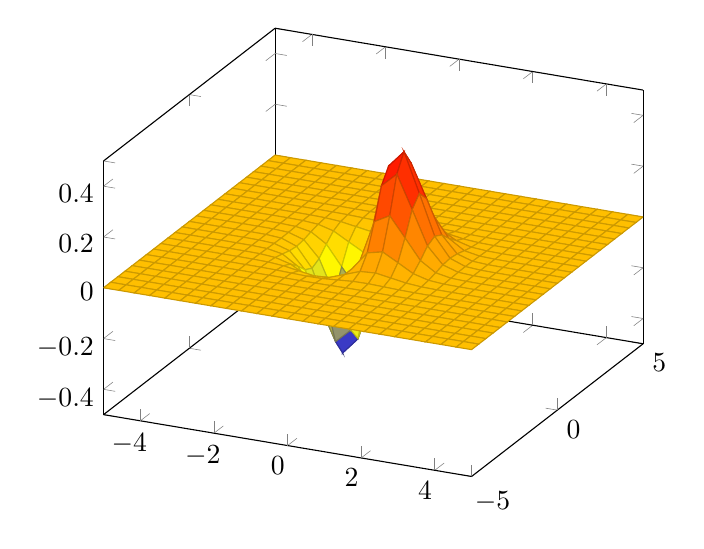
\begin{tikzpicture}
\begin{axis}
\addplot3[
    surf,
]
{exp(-x^2-y^2)*x};
\end{axis}
\end{tikzpicture}

% mesh was my guess
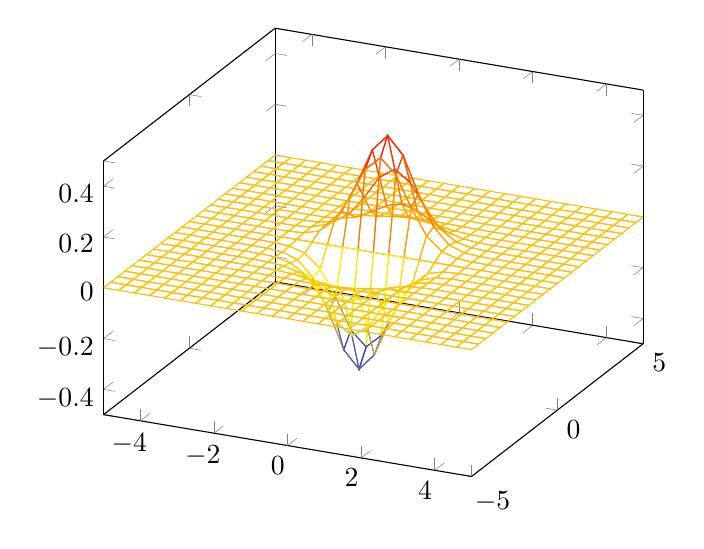
\begin{tikzpicture}
\begin{axis}
\addplot3[
    mesh,
]
{exp(-x^2-y^2)*y};
\end{axis}
\end{tikzpicture}

\begin{figure}
\centering
%% Creator: Matplotlib, PGF backend
%%
%% To include the figure in your LaTeX document, write
%%   \input{<filename>.pgf}
%%
%% Make sure the required packages are loaded in your preamble
%%   \usepackage{pgf}
%%
%% Figures using additional raster images can only be included by \input if
%% they are in the same directory as the main LaTeX file. For loading figures
%% from other directories you can use the `import` package
%%   \usepackage{import}
%% and then include the figures with
%%   \import{<path to file>}{<filename>.pgf}
%%
%% Matplotlib used the following preamble
%%   \usepackage{fontspec}
%%   \setmainfont{DejaVuSerif.ttf}[Path=/home/tgandor/anaconda3/lib/python3.7/site-packages/matplotlib/mpl-data/fonts/ttf/]
%%   \setsansfont{DejaVuSans.ttf}[Path=/home/tgandor/anaconda3/lib/python3.7/site-packages/matplotlib/mpl-data/fonts/ttf/]
%%   \setmonofont{DejaVuSansMono.ttf}[Path=/home/tgandor/anaconda3/lib/python3.7/site-packages/matplotlib/mpl-data/fonts/ttf/]
%%
\begingroup%
\makeatletter%
\begin{pgfpicture}%
\pgfpathrectangle{\pgfpointorigin}{\pgfqpoint{3.000000in}{2.000000in}}%
\pgfusepath{use as bounding box, clip}%
\begin{pgfscope}%
\pgfsetbuttcap%
\pgfsetmiterjoin%
\definecolor{currentfill}{rgb}{1.000000,1.000000,1.000000}%
\pgfsetfillcolor{currentfill}%
\pgfsetlinewidth{0.000000pt}%
\definecolor{currentstroke}{rgb}{1.000000,1.000000,1.000000}%
\pgfsetstrokecolor{currentstroke}%
\pgfsetdash{}{0pt}%
\pgfpathmoveto{\pgfqpoint{0.000000in}{0.000000in}}%
\pgfpathlineto{\pgfqpoint{3.000000in}{0.000000in}}%
\pgfpathlineto{\pgfqpoint{3.000000in}{2.000000in}}%
\pgfpathlineto{\pgfqpoint{0.000000in}{2.000000in}}%
\pgfpathclose%
\pgfusepath{fill}%
\end{pgfscope}%
\begin{pgfscope}%
\pgfsetbuttcap%
\pgfsetmiterjoin%
\definecolor{currentfill}{rgb}{1.000000,1.000000,1.000000}%
\pgfsetfillcolor{currentfill}%
\pgfsetlinewidth{0.000000pt}%
\definecolor{currentstroke}{rgb}{0.000000,0.000000,0.000000}%
\pgfsetstrokecolor{currentstroke}%
\pgfsetstrokeopacity{0.000000}%
\pgfsetdash{}{0pt}%
\pgfpathmoveto{\pgfqpoint{0.375000in}{0.250000in}}%
\pgfpathlineto{\pgfqpoint{2.700000in}{0.250000in}}%
\pgfpathlineto{\pgfqpoint{2.700000in}{1.760000in}}%
\pgfpathlineto{\pgfqpoint{0.375000in}{1.760000in}}%
\pgfpathclose%
\pgfusepath{fill}%
\end{pgfscope}%
\begin{pgfscope}%
\pgfsetbuttcap%
\pgfsetroundjoin%
\definecolor{currentfill}{rgb}{0.000000,0.000000,0.000000}%
\pgfsetfillcolor{currentfill}%
\pgfsetlinewidth{0.803000pt}%
\definecolor{currentstroke}{rgb}{0.000000,0.000000,0.000000}%
\pgfsetstrokecolor{currentstroke}%
\pgfsetdash{}{0pt}%
\pgfsys@defobject{currentmarker}{\pgfqpoint{0.000000in}{-0.048611in}}{\pgfqpoint{0.000000in}{0.000000in}}{%
\pgfpathmoveto{\pgfqpoint{0.000000in}{0.000000in}}%
\pgfpathlineto{\pgfqpoint{0.000000in}{-0.048611in}}%
\pgfusepath{stroke,fill}%
}%
\begin{pgfscope}%
\pgfsys@transformshift{0.459332in}{0.250000in}%
\pgfsys@useobject{currentmarker}{}%
\end{pgfscope}%
\end{pgfscope}%
\begin{pgfscope}%
\definecolor{textcolor}{rgb}{0.000000,0.000000,0.000000}%
\pgfsetstrokecolor{textcolor}%
\pgfsetfillcolor{textcolor}%
\pgftext[x=0.459332in,y=0.152778in,,top]{\color{textcolor}\sffamily\fontsize{10.000000}{12.000000}\selectfont 0}%
\end{pgfscope}%
\begin{pgfscope}%
\pgfsetbuttcap%
\pgfsetroundjoin%
\definecolor{currentfill}{rgb}{0.000000,0.000000,0.000000}%
\pgfsetfillcolor{currentfill}%
\pgfsetlinewidth{0.803000pt}%
\definecolor{currentstroke}{rgb}{0.000000,0.000000,0.000000}%
\pgfsetstrokecolor{currentstroke}%
\pgfsetdash{}{0pt}%
\pgfsys@defobject{currentmarker}{\pgfqpoint{0.000000in}{-0.048611in}}{\pgfqpoint{0.000000in}{0.000000in}}{%
\pgfpathmoveto{\pgfqpoint{0.000000in}{0.000000in}}%
\pgfpathlineto{\pgfqpoint{0.000000in}{-0.048611in}}%
\pgfusepath{stroke,fill}%
}%
\begin{pgfscope}%
\pgfsys@transformshift{0.993079in}{0.250000in}%
\pgfsys@useobject{currentmarker}{}%
\end{pgfscope}%
\end{pgfscope}%
\begin{pgfscope}%
\definecolor{textcolor}{rgb}{0.000000,0.000000,0.000000}%
\pgfsetstrokecolor{textcolor}%
\pgfsetfillcolor{textcolor}%
\pgftext[x=0.993079in,y=0.152778in,,top]{\color{textcolor}\sffamily\fontsize{10.000000}{12.000000}\selectfont 25}%
\end{pgfscope}%
\begin{pgfscope}%
\pgfsetbuttcap%
\pgfsetroundjoin%
\definecolor{currentfill}{rgb}{0.000000,0.000000,0.000000}%
\pgfsetfillcolor{currentfill}%
\pgfsetlinewidth{0.803000pt}%
\definecolor{currentstroke}{rgb}{0.000000,0.000000,0.000000}%
\pgfsetstrokecolor{currentstroke}%
\pgfsetdash{}{0pt}%
\pgfsys@defobject{currentmarker}{\pgfqpoint{0.000000in}{-0.048611in}}{\pgfqpoint{0.000000in}{0.000000in}}{%
\pgfpathmoveto{\pgfqpoint{0.000000in}{0.000000in}}%
\pgfpathlineto{\pgfqpoint{0.000000in}{-0.048611in}}%
\pgfusepath{stroke,fill}%
}%
\begin{pgfscope}%
\pgfsys@transformshift{1.526825in}{0.250000in}%
\pgfsys@useobject{currentmarker}{}%
\end{pgfscope}%
\end{pgfscope}%
\begin{pgfscope}%
\definecolor{textcolor}{rgb}{0.000000,0.000000,0.000000}%
\pgfsetstrokecolor{textcolor}%
\pgfsetfillcolor{textcolor}%
\pgftext[x=1.526825in,y=0.152778in,,top]{\color{textcolor}\sffamily\fontsize{10.000000}{12.000000}\selectfont 50}%
\end{pgfscope}%
\begin{pgfscope}%
\pgfsetbuttcap%
\pgfsetroundjoin%
\definecolor{currentfill}{rgb}{0.000000,0.000000,0.000000}%
\pgfsetfillcolor{currentfill}%
\pgfsetlinewidth{0.803000pt}%
\definecolor{currentstroke}{rgb}{0.000000,0.000000,0.000000}%
\pgfsetstrokecolor{currentstroke}%
\pgfsetdash{}{0pt}%
\pgfsys@defobject{currentmarker}{\pgfqpoint{0.000000in}{-0.048611in}}{\pgfqpoint{0.000000in}{0.000000in}}{%
\pgfpathmoveto{\pgfqpoint{0.000000in}{0.000000in}}%
\pgfpathlineto{\pgfqpoint{0.000000in}{-0.048611in}}%
\pgfusepath{stroke,fill}%
}%
\begin{pgfscope}%
\pgfsys@transformshift{2.060572in}{0.250000in}%
\pgfsys@useobject{currentmarker}{}%
\end{pgfscope}%
\end{pgfscope}%
\begin{pgfscope}%
\definecolor{textcolor}{rgb}{0.000000,0.000000,0.000000}%
\pgfsetstrokecolor{textcolor}%
\pgfsetfillcolor{textcolor}%
\pgftext[x=2.060572in,y=0.152778in,,top]{\color{textcolor}\sffamily\fontsize{10.000000}{12.000000}\selectfont 75}%
\end{pgfscope}%
\begin{pgfscope}%
\pgfsetbuttcap%
\pgfsetroundjoin%
\definecolor{currentfill}{rgb}{0.000000,0.000000,0.000000}%
\pgfsetfillcolor{currentfill}%
\pgfsetlinewidth{0.803000pt}%
\definecolor{currentstroke}{rgb}{0.000000,0.000000,0.000000}%
\pgfsetstrokecolor{currentstroke}%
\pgfsetdash{}{0pt}%
\pgfsys@defobject{currentmarker}{\pgfqpoint{0.000000in}{-0.048611in}}{\pgfqpoint{0.000000in}{0.000000in}}{%
\pgfpathmoveto{\pgfqpoint{0.000000in}{0.000000in}}%
\pgfpathlineto{\pgfqpoint{0.000000in}{-0.048611in}}%
\pgfusepath{stroke,fill}%
}%
\begin{pgfscope}%
\pgfsys@transformshift{2.594318in}{0.250000in}%
\pgfsys@useobject{currentmarker}{}%
\end{pgfscope}%
\end{pgfscope}%
\begin{pgfscope}%
\definecolor{textcolor}{rgb}{0.000000,0.000000,0.000000}%
\pgfsetstrokecolor{textcolor}%
\pgfsetfillcolor{textcolor}%
\pgftext[x=2.594318in,y=0.152778in,,top]{\color{textcolor}\sffamily\fontsize{10.000000}{12.000000}\selectfont 100}%
\end{pgfscope}%
\begin{pgfscope}%
\definecolor{textcolor}{rgb}{0.000000,0.000000,0.000000}%
\pgfsetstrokecolor{textcolor}%
\pgfsetfillcolor{textcolor}%
\pgftext[x=1.537500in,y=-0.037191in,,top]{\color{textcolor}\sffamily\fontsize{10.000000}{12.000000}\selectfont q}%
\end{pgfscope}%
\begin{pgfscope}%
\pgfsetbuttcap%
\pgfsetroundjoin%
\definecolor{currentfill}{rgb}{0.000000,0.000000,0.000000}%
\pgfsetfillcolor{currentfill}%
\pgfsetlinewidth{0.803000pt}%
\definecolor{currentstroke}{rgb}{0.000000,0.000000,0.000000}%
\pgfsetstrokecolor{currentstroke}%
\pgfsetdash{}{0pt}%
\pgfsys@defobject{currentmarker}{\pgfqpoint{-0.048611in}{0.000000in}}{\pgfqpoint{0.000000in}{0.000000in}}{%
\pgfpathmoveto{\pgfqpoint{0.000000in}{0.000000in}}%
\pgfpathlineto{\pgfqpoint{-0.048611in}{0.000000in}}%
\pgfusepath{stroke,fill}%
}%
\begin{pgfscope}%
\pgfsys@transformshift{0.375000in}{0.300492in}%
\pgfsys@useobject{currentmarker}{}%
\end{pgfscope}%
\end{pgfscope}%
\begin{pgfscope}%
\definecolor{textcolor}{rgb}{0.000000,0.000000,0.000000}%
\pgfsetstrokecolor{textcolor}%
\pgfsetfillcolor{textcolor}%
\pgftext[x=0.189412in,y=0.247731in,left,base]{\color{textcolor}\sffamily\fontsize{10.000000}{12.000000}\selectfont 0}%
\end{pgfscope}%
\begin{pgfscope}%
\pgfsetbuttcap%
\pgfsetroundjoin%
\definecolor{currentfill}{rgb}{0.000000,0.000000,0.000000}%
\pgfsetfillcolor{currentfill}%
\pgfsetlinewidth{0.803000pt}%
\definecolor{currentstroke}{rgb}{0.000000,0.000000,0.000000}%
\pgfsetstrokecolor{currentstroke}%
\pgfsetdash{}{0pt}%
\pgfsys@defobject{currentmarker}{\pgfqpoint{-0.048611in}{0.000000in}}{\pgfqpoint{0.000000in}{0.000000in}}{%
\pgfpathmoveto{\pgfqpoint{0.000000in}{0.000000in}}%
\pgfpathlineto{\pgfqpoint{-0.048611in}{0.000000in}}%
\pgfusepath{stroke,fill}%
}%
\begin{pgfscope}%
\pgfsys@transformshift{0.375000in}{0.809987in}%
\pgfsys@useobject{currentmarker}{}%
\end{pgfscope}%
\end{pgfscope}%
\begin{pgfscope}%
\definecolor{textcolor}{rgb}{0.000000,0.000000,0.000000}%
\pgfsetstrokecolor{textcolor}%
\pgfsetfillcolor{textcolor}%
\pgftext[x=0.101047in,y=0.757226in,left,base]{\color{textcolor}\sffamily\fontsize{10.000000}{12.000000}\selectfont 20}%
\end{pgfscope}%
\begin{pgfscope}%
\pgfsetbuttcap%
\pgfsetroundjoin%
\definecolor{currentfill}{rgb}{0.000000,0.000000,0.000000}%
\pgfsetfillcolor{currentfill}%
\pgfsetlinewidth{0.803000pt}%
\definecolor{currentstroke}{rgb}{0.000000,0.000000,0.000000}%
\pgfsetstrokecolor{currentstroke}%
\pgfsetdash{}{0pt}%
\pgfsys@defobject{currentmarker}{\pgfqpoint{-0.048611in}{0.000000in}}{\pgfqpoint{0.000000in}{0.000000in}}{%
\pgfpathmoveto{\pgfqpoint{0.000000in}{0.000000in}}%
\pgfpathlineto{\pgfqpoint{-0.048611in}{0.000000in}}%
\pgfusepath{stroke,fill}%
}%
\begin{pgfscope}%
\pgfsys@transformshift{0.375000in}{1.319483in}%
\pgfsys@useobject{currentmarker}{}%
\end{pgfscope}%
\end{pgfscope}%
\begin{pgfscope}%
\definecolor{textcolor}{rgb}{0.000000,0.000000,0.000000}%
\pgfsetstrokecolor{textcolor}%
\pgfsetfillcolor{textcolor}%
\pgftext[x=0.101047in,y=1.266721in,left,base]{\color{textcolor}\sffamily\fontsize{10.000000}{12.000000}\selectfont 40}%
\end{pgfscope}%
\begin{pgfscope}%
\pgfpathrectangle{\pgfqpoint{0.375000in}{0.250000in}}{\pgfqpoint{2.325000in}{1.510000in}}%
\pgfusepath{clip}%
\pgfsetrectcap%
\pgfsetroundjoin%
\pgfsetlinewidth{1.505625pt}%
\definecolor{currentstroke}{rgb}{0.121569,0.466667,0.705882}%
\pgfsetstrokecolor{currentstroke}%
\pgfsetdash{}{0pt}%
\pgfpathmoveto{\pgfqpoint{0.480682in}{0.333051in}}%
\pgfpathlineto{\pgfqpoint{0.502032in}{0.332972in}}%
\pgfpathlineto{\pgfqpoint{0.523382in}{0.344167in}}%
\pgfpathlineto{\pgfqpoint{0.544731in}{0.374174in}}%
\pgfpathlineto{\pgfqpoint{0.566081in}{0.422363in}}%
\pgfpathlineto{\pgfqpoint{0.587431in}{0.487016in}}%
\pgfpathlineto{\pgfqpoint{0.608781in}{0.550899in}}%
\pgfpathlineto{\pgfqpoint{0.630131in}{0.624941in}}%
\pgfpathlineto{\pgfqpoint{0.651481in}{0.700958in}}%
\pgfpathlineto{\pgfqpoint{0.672831in}{0.770656in}}%
\pgfpathlineto{\pgfqpoint{0.694180in}{0.834159in}}%
\pgfpathlineto{\pgfqpoint{0.715530in}{0.902793in}}%
\pgfpathlineto{\pgfqpoint{0.736880in}{0.967534in}}%
\pgfpathlineto{\pgfqpoint{0.758230in}{1.018110in}}%
\pgfpathlineto{\pgfqpoint{0.779580in}{1.076164in}}%
\pgfpathlineto{\pgfqpoint{0.800930in}{1.128663in}}%
\pgfpathlineto{\pgfqpoint{0.822280in}{1.172628in}}%
\pgfpathlineto{\pgfqpoint{0.843629in}{1.214833in}}%
\pgfpathlineto{\pgfqpoint{0.864979in}{1.241071in}}%
\pgfpathlineto{\pgfqpoint{0.886329in}{1.281803in}}%
\pgfpathlineto{\pgfqpoint{0.907679in}{1.306786in}}%
\pgfpathlineto{\pgfqpoint{0.929029in}{1.325011in}}%
\pgfpathlineto{\pgfqpoint{0.950379in}{1.355082in}}%
\pgfpathlineto{\pgfqpoint{0.971729in}{1.386842in}}%
\pgfpathlineto{\pgfqpoint{0.993079in}{1.390686in}}%
\pgfpathlineto{\pgfqpoint{1.014428in}{1.408070in}}%
\pgfpathlineto{\pgfqpoint{1.035778in}{1.424634in}}%
\pgfpathlineto{\pgfqpoint{1.057128in}{1.439918in}}%
\pgfpathlineto{\pgfqpoint{1.078478in}{1.445362in}}%
\pgfpathlineto{\pgfqpoint{1.099828in}{1.462995in}}%
\pgfpathlineto{\pgfqpoint{1.121178in}{1.465015in}}%
\pgfpathlineto{\pgfqpoint{1.142528in}{1.472072in}}%
\pgfpathlineto{\pgfqpoint{1.163877in}{1.485534in}}%
\pgfpathlineto{\pgfqpoint{1.185227in}{1.490526in}}%
\pgfpathlineto{\pgfqpoint{1.206577in}{1.501875in}}%
\pgfpathlineto{\pgfqpoint{1.227927in}{1.504529in}}%
\pgfpathlineto{\pgfqpoint{1.249277in}{1.511217in}}%
\pgfpathlineto{\pgfqpoint{1.270627in}{1.522875in}}%
\pgfpathlineto{\pgfqpoint{1.291977in}{1.529248in}}%
\pgfpathlineto{\pgfqpoint{1.313326in}{1.532270in}}%
\pgfpathlineto{\pgfqpoint{1.334676in}{1.538331in}}%
\pgfpathlineto{\pgfqpoint{1.356026in}{1.539480in}}%
\pgfpathlineto{\pgfqpoint{1.377376in}{1.549952in}}%
\pgfpathlineto{\pgfqpoint{1.398726in}{1.557241in}}%
\pgfpathlineto{\pgfqpoint{1.420076in}{1.562352in}}%
\pgfpathlineto{\pgfqpoint{1.441426in}{1.564752in}}%
\pgfpathlineto{\pgfqpoint{1.462775in}{1.565653in}}%
\pgfpathlineto{\pgfqpoint{1.484125in}{1.571579in}}%
\pgfpathlineto{\pgfqpoint{1.505475in}{1.572315in}}%
\pgfpathlineto{\pgfqpoint{1.526825in}{1.573969in}}%
\pgfpathlineto{\pgfqpoint{1.548175in}{1.576759in}}%
\pgfpathlineto{\pgfqpoint{1.569525in}{1.581823in}}%
\pgfpathlineto{\pgfqpoint{1.590875in}{1.585460in}}%
\pgfpathlineto{\pgfqpoint{1.612225in}{1.588739in}}%
\pgfpathlineto{\pgfqpoint{1.633574in}{1.587801in}}%
\pgfpathlineto{\pgfqpoint{1.654924in}{1.592597in}}%
\pgfpathlineto{\pgfqpoint{1.676274in}{1.593530in}}%
\pgfpathlineto{\pgfqpoint{1.697624in}{1.599584in}}%
\pgfpathlineto{\pgfqpoint{1.718974in}{1.598392in}}%
\pgfpathlineto{\pgfqpoint{1.740324in}{1.600765in}}%
\pgfpathlineto{\pgfqpoint{1.761674in}{1.603105in}}%
\pgfpathlineto{\pgfqpoint{1.783023in}{1.606642in}}%
\pgfpathlineto{\pgfqpoint{1.804373in}{1.609288in}}%
\pgfpathlineto{\pgfqpoint{1.825723in}{1.609926in}}%
\pgfpathlineto{\pgfqpoint{1.847073in}{1.617878in}}%
\pgfpathlineto{\pgfqpoint{1.868423in}{1.621265in}}%
\pgfpathlineto{\pgfqpoint{1.889773in}{1.624049in}}%
\pgfpathlineto{\pgfqpoint{1.911123in}{1.625716in}}%
\pgfpathlineto{\pgfqpoint{1.932472in}{1.628595in}}%
\pgfpathlineto{\pgfqpoint{1.953822in}{1.628264in}}%
\pgfpathlineto{\pgfqpoint{1.975172in}{1.635462in}}%
\pgfpathlineto{\pgfqpoint{1.996522in}{1.639488in}}%
\pgfpathlineto{\pgfqpoint{2.017872in}{1.638926in}}%
\pgfpathlineto{\pgfqpoint{2.039222in}{1.641271in}}%
\pgfpathlineto{\pgfqpoint{2.060572in}{1.641679in}}%
\pgfpathlineto{\pgfqpoint{2.081921in}{1.643658in}}%
\pgfpathlineto{\pgfqpoint{2.103271in}{1.645056in}}%
\pgfpathlineto{\pgfqpoint{2.124621in}{1.651185in}}%
\pgfpathlineto{\pgfqpoint{2.145971in}{1.652289in}}%
\pgfpathlineto{\pgfqpoint{2.167321in}{1.650287in}}%
\pgfpathlineto{\pgfqpoint{2.188671in}{1.652225in}}%
\pgfpathlineto{\pgfqpoint{2.210021in}{1.655143in}}%
\pgfpathlineto{\pgfqpoint{2.231371in}{1.659020in}}%
\pgfpathlineto{\pgfqpoint{2.252720in}{1.660957in}}%
\pgfpathlineto{\pgfqpoint{2.274070in}{1.664829in}}%
\pgfpathlineto{\pgfqpoint{2.295420in}{1.668974in}}%
\pgfpathlineto{\pgfqpoint{2.316770in}{1.669948in}}%
\pgfpathlineto{\pgfqpoint{2.338120in}{1.675786in}}%
\pgfpathlineto{\pgfqpoint{2.359470in}{1.679481in}}%
\pgfpathlineto{\pgfqpoint{2.380820in}{1.678036in}}%
\pgfpathlineto{\pgfqpoint{2.402169in}{1.681913in}}%
\pgfpathlineto{\pgfqpoint{2.423519in}{1.680584in}}%
\pgfpathlineto{\pgfqpoint{2.444869in}{1.684933in}}%
\pgfpathlineto{\pgfqpoint{2.466219in}{1.687248in}}%
\pgfpathlineto{\pgfqpoint{2.487569in}{1.688365in}}%
\pgfpathlineto{\pgfqpoint{2.508919in}{1.689089in}}%
\pgfpathlineto{\pgfqpoint{2.530269in}{1.685916in}}%
\pgfpathlineto{\pgfqpoint{2.551618in}{1.688786in}}%
\pgfpathlineto{\pgfqpoint{2.572968in}{1.690464in}}%
\pgfpathlineto{\pgfqpoint{2.594318in}{1.691364in}}%
\pgfusepath{stroke}%
\end{pgfscope}%
\begin{pgfscope}%
\pgfpathrectangle{\pgfqpoint{0.375000in}{0.250000in}}{\pgfqpoint{2.325000in}{1.510000in}}%
\pgfusepath{clip}%
\pgfsetrectcap%
\pgfsetroundjoin%
\pgfsetlinewidth{1.505625pt}%
\definecolor{currentstroke}{rgb}{1.000000,0.498039,0.054902}%
\pgfsetstrokecolor{currentstroke}%
\pgfsetdash{}{0pt}%
\pgfpathmoveto{\pgfqpoint{0.480682in}{0.318636in}}%
\pgfpathlineto{\pgfqpoint{0.502032in}{0.318639in}}%
\pgfpathlineto{\pgfqpoint{0.523382in}{0.325153in}}%
\pgfpathlineto{\pgfqpoint{0.544731in}{0.342257in}}%
\pgfpathlineto{\pgfqpoint{0.566081in}{0.374661in}}%
\pgfpathlineto{\pgfqpoint{0.587431in}{0.412911in}}%
\pgfpathlineto{\pgfqpoint{0.608781in}{0.452672in}}%
\pgfpathlineto{\pgfqpoint{0.630131in}{0.497185in}}%
\pgfpathlineto{\pgfqpoint{0.651481in}{0.545489in}}%
\pgfpathlineto{\pgfqpoint{0.672831in}{0.594181in}}%
\pgfpathlineto{\pgfqpoint{0.694180in}{0.634815in}}%
\pgfpathlineto{\pgfqpoint{0.715530in}{0.677086in}}%
\pgfpathlineto{\pgfqpoint{0.736880in}{0.721334in}}%
\pgfpathlineto{\pgfqpoint{0.758230in}{0.753895in}}%
\pgfpathlineto{\pgfqpoint{0.779580in}{0.794054in}}%
\pgfpathlineto{\pgfqpoint{0.800930in}{0.829105in}}%
\pgfpathlineto{\pgfqpoint{0.822280in}{0.859887in}}%
\pgfpathlineto{\pgfqpoint{0.843629in}{0.888874in}}%
\pgfpathlineto{\pgfqpoint{0.864979in}{0.911009in}}%
\pgfpathlineto{\pgfqpoint{0.886329in}{0.933333in}}%
\pgfpathlineto{\pgfqpoint{0.907679in}{0.956096in}}%
\pgfpathlineto{\pgfqpoint{0.929029in}{0.968697in}}%
\pgfpathlineto{\pgfqpoint{0.950379in}{0.990950in}}%
\pgfpathlineto{\pgfqpoint{0.971729in}{1.014758in}}%
\pgfpathlineto{\pgfqpoint{0.993079in}{1.019496in}}%
\pgfpathlineto{\pgfqpoint{1.014428in}{1.030744in}}%
\pgfpathlineto{\pgfqpoint{1.035778in}{1.046087in}}%
\pgfpathlineto{\pgfqpoint{1.057128in}{1.059466in}}%
\pgfpathlineto{\pgfqpoint{1.078478in}{1.063707in}}%
\pgfpathlineto{\pgfqpoint{1.099828in}{1.076357in}}%
\pgfpathlineto{\pgfqpoint{1.121178in}{1.077849in}}%
\pgfpathlineto{\pgfqpoint{1.142528in}{1.084056in}}%
\pgfpathlineto{\pgfqpoint{1.163877in}{1.094745in}}%
\pgfpathlineto{\pgfqpoint{1.185227in}{1.097543in}}%
\pgfpathlineto{\pgfqpoint{1.206577in}{1.107089in}}%
\pgfpathlineto{\pgfqpoint{1.227927in}{1.109415in}}%
\pgfpathlineto{\pgfqpoint{1.249277in}{1.115661in}}%
\pgfpathlineto{\pgfqpoint{1.270627in}{1.122948in}}%
\pgfpathlineto{\pgfqpoint{1.291977in}{1.126514in}}%
\pgfpathlineto{\pgfqpoint{1.313326in}{1.131858in}}%
\pgfpathlineto{\pgfqpoint{1.334676in}{1.134165in}}%
\pgfpathlineto{\pgfqpoint{1.356026in}{1.137314in}}%
\pgfpathlineto{\pgfqpoint{1.377376in}{1.142880in}}%
\pgfpathlineto{\pgfqpoint{1.398726in}{1.149438in}}%
\pgfpathlineto{\pgfqpoint{1.420076in}{1.150573in}}%
\pgfpathlineto{\pgfqpoint{1.441426in}{1.153365in}}%
\pgfpathlineto{\pgfqpoint{1.462775in}{1.153004in}}%
\pgfpathlineto{\pgfqpoint{1.484125in}{1.157193in}}%
\pgfpathlineto{\pgfqpoint{1.505475in}{1.158865in}}%
\pgfpathlineto{\pgfqpoint{1.526825in}{1.160914in}}%
\pgfpathlineto{\pgfqpoint{1.548175in}{1.161868in}}%
\pgfpathlineto{\pgfqpoint{1.569525in}{1.167108in}}%
\pgfpathlineto{\pgfqpoint{1.590875in}{1.171320in}}%
\pgfpathlineto{\pgfqpoint{1.612225in}{1.174332in}}%
\pgfpathlineto{\pgfqpoint{1.633574in}{1.171701in}}%
\pgfpathlineto{\pgfqpoint{1.654924in}{1.174077in}}%
\pgfpathlineto{\pgfqpoint{1.676274in}{1.177085in}}%
\pgfpathlineto{\pgfqpoint{1.697624in}{1.182232in}}%
\pgfpathlineto{\pgfqpoint{1.718974in}{1.181978in}}%
\pgfpathlineto{\pgfqpoint{1.740324in}{1.181998in}}%
\pgfpathlineto{\pgfqpoint{1.761674in}{1.183093in}}%
\pgfpathlineto{\pgfqpoint{1.783023in}{1.188788in}}%
\pgfpathlineto{\pgfqpoint{1.804373in}{1.186556in}}%
\pgfpathlineto{\pgfqpoint{1.825723in}{1.188452in}}%
\pgfpathlineto{\pgfqpoint{1.847073in}{1.196319in}}%
\pgfpathlineto{\pgfqpoint{1.868423in}{1.199560in}}%
\pgfpathlineto{\pgfqpoint{1.889773in}{1.202081in}}%
\pgfpathlineto{\pgfqpoint{1.911123in}{1.203718in}}%
\pgfpathlineto{\pgfqpoint{1.932472in}{1.203102in}}%
\pgfpathlineto{\pgfqpoint{1.953822in}{1.207167in}}%
\pgfpathlineto{\pgfqpoint{1.975172in}{1.208632in}}%
\pgfpathlineto{\pgfqpoint{1.996522in}{1.211239in}}%
\pgfpathlineto{\pgfqpoint{2.017872in}{1.212991in}}%
\pgfpathlineto{\pgfqpoint{2.039222in}{1.215097in}}%
\pgfpathlineto{\pgfqpoint{2.060572in}{1.213787in}}%
\pgfpathlineto{\pgfqpoint{2.081921in}{1.215841in}}%
\pgfpathlineto{\pgfqpoint{2.103271in}{1.219141in}}%
\pgfpathlineto{\pgfqpoint{2.124621in}{1.223650in}}%
\pgfpathlineto{\pgfqpoint{2.145971in}{1.223523in}}%
\pgfpathlineto{\pgfqpoint{2.167321in}{1.223164in}}%
\pgfpathlineto{\pgfqpoint{2.188671in}{1.225864in}}%
\pgfpathlineto{\pgfqpoint{2.210021in}{1.228287in}}%
\pgfpathlineto{\pgfqpoint{2.231371in}{1.230867in}}%
\pgfpathlineto{\pgfqpoint{2.252720in}{1.231847in}}%
\pgfpathlineto{\pgfqpoint{2.274070in}{1.235275in}}%
\pgfpathlineto{\pgfqpoint{2.295420in}{1.236729in}}%
\pgfpathlineto{\pgfqpoint{2.316770in}{1.239036in}}%
\pgfpathlineto{\pgfqpoint{2.338120in}{1.242876in}}%
\pgfpathlineto{\pgfqpoint{2.359470in}{1.244789in}}%
\pgfpathlineto{\pgfqpoint{2.380820in}{1.245728in}}%
\pgfpathlineto{\pgfqpoint{2.402169in}{1.246684in}}%
\pgfpathlineto{\pgfqpoint{2.423519in}{1.246437in}}%
\pgfpathlineto{\pgfqpoint{2.444869in}{1.249926in}}%
\pgfpathlineto{\pgfqpoint{2.466219in}{1.249894in}}%
\pgfpathlineto{\pgfqpoint{2.487569in}{1.253444in}}%
\pgfpathlineto{\pgfqpoint{2.508919in}{1.254326in}}%
\pgfpathlineto{\pgfqpoint{2.530269in}{1.251430in}}%
\pgfpathlineto{\pgfqpoint{2.551618in}{1.252937in}}%
\pgfpathlineto{\pgfqpoint{2.572968in}{1.254753in}}%
\pgfpathlineto{\pgfqpoint{2.594318in}{1.254950in}}%
\pgfusepath{stroke}%
\end{pgfscope}%
\begin{pgfscope}%
\pgfsetrectcap%
\pgfsetmiterjoin%
\pgfsetlinewidth{0.803000pt}%
\definecolor{currentstroke}{rgb}{0.000000,0.000000,0.000000}%
\pgfsetstrokecolor{currentstroke}%
\pgfsetdash{}{0pt}%
\pgfpathmoveto{\pgfqpoint{0.375000in}{0.250000in}}%
\pgfpathlineto{\pgfqpoint{0.375000in}{1.760000in}}%
\pgfusepath{stroke}%
\end{pgfscope}%
\begin{pgfscope}%
\pgfsetrectcap%
\pgfsetmiterjoin%
\pgfsetlinewidth{0.803000pt}%
\definecolor{currentstroke}{rgb}{0.000000,0.000000,0.000000}%
\pgfsetstrokecolor{currentstroke}%
\pgfsetdash{}{0pt}%
\pgfpathmoveto{\pgfqpoint{2.700000in}{0.250000in}}%
\pgfpathlineto{\pgfqpoint{2.700000in}{1.760000in}}%
\pgfusepath{stroke}%
\end{pgfscope}%
\begin{pgfscope}%
\pgfsetrectcap%
\pgfsetmiterjoin%
\pgfsetlinewidth{0.803000pt}%
\definecolor{currentstroke}{rgb}{0.000000,0.000000,0.000000}%
\pgfsetstrokecolor{currentstroke}%
\pgfsetdash{}{0pt}%
\pgfpathmoveto{\pgfqpoint{0.375000in}{0.250000in}}%
\pgfpathlineto{\pgfqpoint{2.700000in}{0.250000in}}%
\pgfusepath{stroke}%
\end{pgfscope}%
\begin{pgfscope}%
\pgfsetrectcap%
\pgfsetmiterjoin%
\pgfsetlinewidth{0.803000pt}%
\definecolor{currentstroke}{rgb}{0.000000,0.000000,0.000000}%
\pgfsetstrokecolor{currentstroke}%
\pgfsetdash{}{0pt}%
\pgfpathmoveto{\pgfqpoint{0.375000in}{1.760000in}}%
\pgfpathlineto{\pgfqpoint{2.700000in}{1.760000in}}%
\pgfusepath{stroke}%
\end{pgfscope}%
\begin{pgfscope}%
\pgfsetbuttcap%
\pgfsetmiterjoin%
\definecolor{currentfill}{rgb}{1.000000,1.000000,1.000000}%
\pgfsetfillcolor{currentfill}%
\pgfsetfillopacity{0.800000}%
\pgfsetlinewidth{1.003750pt}%
\definecolor{currentstroke}{rgb}{0.800000,0.800000,0.800000}%
\pgfsetstrokecolor{currentstroke}%
\pgfsetstrokeopacity{0.800000}%
\pgfsetdash{}{0pt}%
\pgfpathmoveto{\pgfqpoint{1.802838in}{0.319444in}}%
\pgfpathlineto{\pgfqpoint{2.602778in}{0.319444in}}%
\pgfpathquadraticcurveto{\pgfqpoint{2.630556in}{0.319444in}}{\pgfqpoint{2.630556in}{0.347222in}}%
\pgfpathlineto{\pgfqpoint{2.630556in}{0.741048in}}%
\pgfpathquadraticcurveto{\pgfqpoint{2.630556in}{0.768826in}}{\pgfqpoint{2.602778in}{0.768826in}}%
\pgfpathlineto{\pgfqpoint{1.802838in}{0.768826in}}%
\pgfpathquadraticcurveto{\pgfqpoint{1.775060in}{0.768826in}}{\pgfqpoint{1.775060in}{0.741048in}}%
\pgfpathlineto{\pgfqpoint{1.775060in}{0.347222in}}%
\pgfpathquadraticcurveto{\pgfqpoint{1.775060in}{0.319444in}}{\pgfqpoint{1.802838in}{0.319444in}}%
\pgfpathclose%
\pgfusepath{stroke,fill}%
\end{pgfscope}%
\begin{pgfscope}%
\pgfsetrectcap%
\pgfsetroundjoin%
\pgfsetlinewidth{1.505625pt}%
\definecolor{currentstroke}{rgb}{0.121569,0.466667,0.705882}%
\pgfsetstrokecolor{currentstroke}%
\pgfsetdash{}{0pt}%
\pgfpathmoveto{\pgfqpoint{1.830615in}{0.656358in}}%
\pgfpathlineto{\pgfqpoint{2.108393in}{0.656358in}}%
\pgfusepath{stroke}%
\end{pgfscope}%
\begin{pgfscope}%
\definecolor{textcolor}{rgb}{0.000000,0.000000,0.000000}%
\pgfsetstrokecolor{textcolor}%
\pgfsetfillcolor{textcolor}%
\pgftext[x=2.219504in,y=0.607747in,left,base]{\color{textcolor}\sffamily\fontsize{10.000000}{12.000000}\selectfont AP50}%
\end{pgfscope}%
\begin{pgfscope}%
\pgfsetrectcap%
\pgfsetroundjoin%
\pgfsetlinewidth{1.505625pt}%
\definecolor{currentstroke}{rgb}{1.000000,0.498039,0.054902}%
\pgfsetstrokecolor{currentstroke}%
\pgfsetdash{}{0pt}%
\pgfpathmoveto{\pgfqpoint{1.830615in}{0.452501in}}%
\pgfpathlineto{\pgfqpoint{2.108393in}{0.452501in}}%
\pgfusepath{stroke}%
\end{pgfscope}%
\begin{pgfscope}%
\definecolor{textcolor}{rgb}{0.000000,0.000000,0.000000}%
\pgfsetstrokecolor{textcolor}%
\pgfsetfillcolor{textcolor}%
\pgftext[x=2.219504in,y=0.403890in,left,base]{\color{textcolor}\sffamily\fontsize{10.000000}{12.000000}\selectfont AP}%
\end{pgfscope}%
\end{pgfpicture}%
\makeatother%
\endgroup%
 
%\includegraphics{wykres2}
\caption{AP and AP50 going up.}
\end{figure}

\begin{figure}
\centering
\begin{tabular}{cc}
  
\includegraphics[width=45mm]{it} &   
\includegraphics[width=45mm]{it} \\
 (a) first & (b) second \\[6pt]
  \null &   
\includegraphics[width=45mm]{it} \\
  \null & (c) right column \\[6pt]
\multicolumn{2}{c}{
\includegraphics[width=45mm]{it} }\\
\multicolumn{2}{c}{(d) centered}
\end{tabular}
\caption{Laying out plots using table (manual)}
\end{figure}

% the Overleaf example:

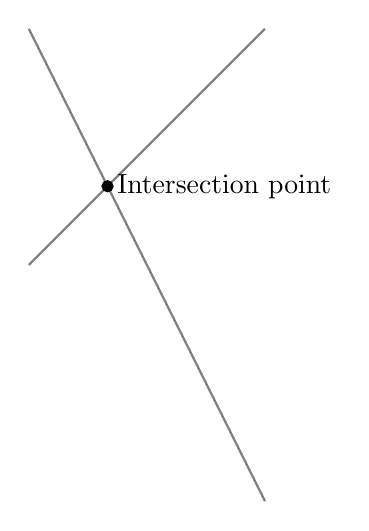
\begin{tikzpicture}
\draw[gray, thick] (-1,2) -- (2,-4);
\draw[gray, thick] (-1,-1) -- (2,2);
\filldraw[black] (0,0) circle (2pt) node[anchor=west] {Intersection point};
\end{tikzpicture}

% https://tex.stackexchange.com/questions/131635/writing-a-backslash-in-the-texttt-environment
First flowchart (requires \verb|\usetikzlibrary{positioning}|, BTW):

\vspace{12pt}

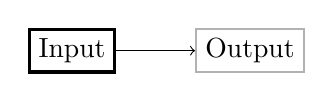
\begin{tikzpicture}[
squarednode/.style={rectangle, draw=black, very thick, minimum size=5mm},
rectnode/.style={rectangle, draw=black!30, thick}, % i.e. gray
]

% Nodes
\node[squarednode] (step1) {Input};
\node[rectnode] (step2) [right=of step1] {Output};

% Arrows
\draw[->] (step1.east) -- (step2.west);

\end{tikzpicture}


\end{document}
